\tikzset{fontscale/.style = {font=\relsize{#1}}
    }
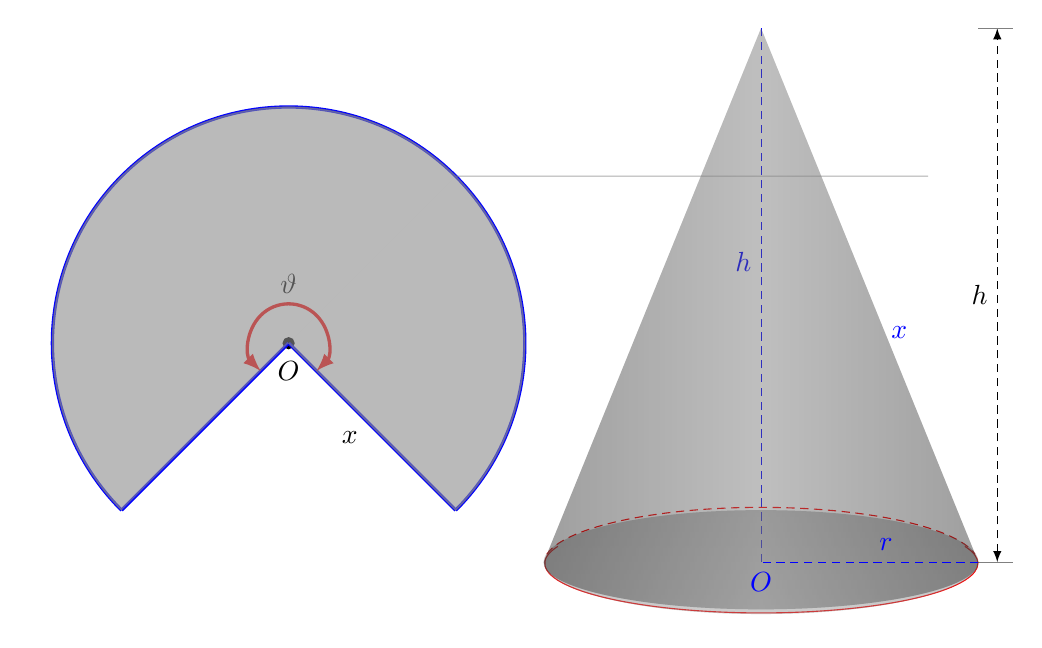
\begin{tikzpicture}[scale=2,
         dot/.style = {
     fill = black!30!brown,
      circle,
      inner sep =2pt,
      minimum size = 4pt
    }
  ]
%%%%%%%%%%%%%%%%%%%%%%%%%%%%%%%%%%%%%%
 %\draw [very thin, style=gray!50, step=0.5] (-4.5,-2) grid (3,2);
 %\draw [thin, gray!60] (0,0) grid (9,9);
\coordinate (O) at (0,0);
\coordinate (O1) at (-3,0);
\coordinate (B1) at (60:1.5);
\coordinate (C1) at (0:-1.5);
%coordinate cone
\coordinate (O) at (0,0);
 \coordinate (A) at (-1.38,1.39);
 \coordinate (B) at (-1.38,-1.39);
 \coordinate (C) at (1.38,1.39);
 \coordinate (D) at (1.38,-1.39);
\coordinate (E) at (0,-1.39);
\coordinate (F) at (0,2);
\coordinate (G) at (1.5,-1.39);
\coordinate (H) at (1.5,2);
\coordinate (I) at (-0.8,0);
\coordinate (J) at (0.8,0);


\filldraw (O1) circle (1pt) node[below=3pt] {$O$};
%%%%%%%%%cone
\draw[color=blue] (J) node[above right=-2pt] {$x$};
   
 \draw[densely dashed,latex-latex] (G) to [edge label = $h$] (H);
  \draw[gray] (D) to (1.6,-1.39);
  \draw[gray] (1.38,2) to (1.6,2);

\draw[densely dashed,blue] (E) to [above=12pt,edge label = $h$] (F);

  % cut of ball surface botton
%  
  \draw[red, densely dashed] (-1.36,-1.34) arc [start angle = 170, end angle = 10,
    x radius = 13.8mm, y radius = 3.6mm];
  \draw[red] (-1.29,-1.29) arc [start angle=-200, end angle = 20,
    x radius = 13.75mm, y radius = 3.15mm];
\fill[
  top color=gray!50,
  bottom color=gray!10,
  shading=axis,
  opacity=0.25
  ] 
  (0,-1.39) circle (1.38cm and 0.33cm);
\fill[
  left color=gray!50!black,
  right color=gray!50!black,
  middle color=gray!50,
  shading=axis,
  opacity=0.25
  ] 
  (1.38,-1.39) -- (0,2) -- (-1.38,-1.39) arc (180:360:1.38cm and 0.3cm);
%%%%%%%%%%%%%%%%%%%%%
% 
%%%%%%%%%%%%%%%%%%%%%5
\draw[densely dashed,blue] (D) to [above=12pt,edge label = $r$] (E);
\draw[color=blue] (0,-1.38) node[below =1pt] {$O$};
%%% circle botton
\draw[blue,very thick] (315:1.5) +(-3,0) -- (-3,0);
\draw[blue,very thick] (225:1.5) +(-3,0) -- (-3,0);
\draw [blue,very thick](225:1.5)++(-3,0.0) arc (225:-45:1.5) ;
\draw (-2.5,-0.5) node[below left] {$x$};
\draw [red,very thick,latex-latex](225:2.5mm)+(-3,0.0) arc (225:-45:2.5mm) ;
\draw (-3,0.5) node[below ] {$\vartheta$};
\shadedraw[ 
draw=gray,
top color=gray!90,
  bottom color=blue!90,
middle color=gray!90,
right color=gray!90,
ball color=blue!90,
  shading=axis,
  opacity=0.60]
  (225:1.5)++(-3,0.0) arc (225:45:1.5);
\shadedraw[ draw=gray,
top color=gray!90,
  bottom color=blue!90,
middle color=gray!90,
right color=gray!90,
ball color=blue!90,
  shading=axis,
  opacity=0.60](45:1.5)++(-3,0)-- (45:1.5)++(-3,0) arc [start angle=45, end angle=-45, radius=1.5] -- (-3,0) ;
  \end{tikzpicture}

%%%%%%%%%%%%%%%%%%%%%%%%%%%%%%%%%%
%%%%%%%%%%%%%%%%%%%%%%%%%%%%%%
